% Options for packages loaded elsewhere
\PassOptionsToPackage{unicode}{hyperref}
\PassOptionsToPackage{hyphens}{url}
\PassOptionsToPackage{dvipsnames,svgnames,x11names}{xcolor}
%
\documentclass[
]{article}
\usepackage{amsmath,amssymb}
\usepackage{iftex}
\ifPDFTeX
  \usepackage[T1]{fontenc}
  \usepackage[utf8]{inputenc}
  \usepackage{textcomp} % provide euro and other symbols
\else % if luatex or xetex
  \usepackage{unicode-math} % this also loads fontspec
  \defaultfontfeatures{Scale=MatchLowercase}
  \defaultfontfeatures[\rmfamily]{Ligatures=TeX,Scale=1}
\fi
\usepackage{lmodern}
\ifPDFTeX\else
  % xetex/luatex font selection
    \setmainfont[]{NanumGothic}
    \setmonofont[]{UnShinmun}
\fi
% Use upquote if available, for straight quotes in verbatim environments
\IfFileExists{upquote.sty}{\usepackage{upquote}}{}
\IfFileExists{microtype.sty}{% use microtype if available
  \usepackage[]{microtype}
  \UseMicrotypeSet[protrusion]{basicmath} % disable protrusion for tt fonts
}{}
\makeatletter
\@ifundefined{KOMAClassName}{% if non-KOMA class
  \IfFileExists{parskip.sty}{%
    \usepackage{parskip}
  }{% else
    \setlength{\parindent}{0pt}
    \setlength{\parskip}{6pt plus 2pt minus 1pt}}
}{% if KOMA class
  \KOMAoptions{parskip=half}}
\makeatother
\usepackage{xcolor}
\usepackage[margin=1in]{geometry}
\usepackage{color}
\usepackage{fancyvrb}
\newcommand{\VerbBar}{|}
\newcommand{\VERB}{\Verb[commandchars=\\\{\}]}
\DefineVerbatimEnvironment{Highlighting}{Verbatim}{commandchars=\\\{\}}
% Add ',fontsize=\small' for more characters per line
\usepackage{framed}
\definecolor{shadecolor}{RGB}{248,248,248}
\newenvironment{Shaded}{\begin{snugshade}}{\end{snugshade}}
\newcommand{\AlertTok}[1]{\textcolor[rgb]{0.94,0.16,0.16}{#1}}
\newcommand{\AnnotationTok}[1]{\textcolor[rgb]{0.56,0.35,0.01}{\textbf{\textit{#1}}}}
\newcommand{\AttributeTok}[1]{\textcolor[rgb]{0.13,0.29,0.53}{#1}}
\newcommand{\BaseNTok}[1]{\textcolor[rgb]{0.00,0.00,0.81}{#1}}
\newcommand{\BuiltInTok}[1]{#1}
\newcommand{\CharTok}[1]{\textcolor[rgb]{0.31,0.60,0.02}{#1}}
\newcommand{\CommentTok}[1]{\textcolor[rgb]{0.56,0.35,0.01}{\textit{#1}}}
\newcommand{\CommentVarTok}[1]{\textcolor[rgb]{0.56,0.35,0.01}{\textbf{\textit{#1}}}}
\newcommand{\ConstantTok}[1]{\textcolor[rgb]{0.56,0.35,0.01}{#1}}
\newcommand{\ControlFlowTok}[1]{\textcolor[rgb]{0.13,0.29,0.53}{\textbf{#1}}}
\newcommand{\DataTypeTok}[1]{\textcolor[rgb]{0.13,0.29,0.53}{#1}}
\newcommand{\DecValTok}[1]{\textcolor[rgb]{0.00,0.00,0.81}{#1}}
\newcommand{\DocumentationTok}[1]{\textcolor[rgb]{0.56,0.35,0.01}{\textbf{\textit{#1}}}}
\newcommand{\ErrorTok}[1]{\textcolor[rgb]{0.64,0.00,0.00}{\textbf{#1}}}
\newcommand{\ExtensionTok}[1]{#1}
\newcommand{\FloatTok}[1]{\textcolor[rgb]{0.00,0.00,0.81}{#1}}
\newcommand{\FunctionTok}[1]{\textcolor[rgb]{0.13,0.29,0.53}{\textbf{#1}}}
\newcommand{\ImportTok}[1]{#1}
\newcommand{\InformationTok}[1]{\textcolor[rgb]{0.56,0.35,0.01}{\textbf{\textit{#1}}}}
\newcommand{\KeywordTok}[1]{\textcolor[rgb]{0.13,0.29,0.53}{\textbf{#1}}}
\newcommand{\NormalTok}[1]{#1}
\newcommand{\OperatorTok}[1]{\textcolor[rgb]{0.81,0.36,0.00}{\textbf{#1}}}
\newcommand{\OtherTok}[1]{\textcolor[rgb]{0.56,0.35,0.01}{#1}}
\newcommand{\PreprocessorTok}[1]{\textcolor[rgb]{0.56,0.35,0.01}{\textit{#1}}}
\newcommand{\RegionMarkerTok}[1]{#1}
\newcommand{\SpecialCharTok}[1]{\textcolor[rgb]{0.81,0.36,0.00}{\textbf{#1}}}
\newcommand{\SpecialStringTok}[1]{\textcolor[rgb]{0.31,0.60,0.02}{#1}}
\newcommand{\StringTok}[1]{\textcolor[rgb]{0.31,0.60,0.02}{#1}}
\newcommand{\VariableTok}[1]{\textcolor[rgb]{0.00,0.00,0.00}{#1}}
\newcommand{\VerbatimStringTok}[1]{\textcolor[rgb]{0.31,0.60,0.02}{#1}}
\newcommand{\WarningTok}[1]{\textcolor[rgb]{0.56,0.35,0.01}{\textbf{\textit{#1}}}}
\usepackage{graphicx}
\makeatletter
\newsavebox\pandoc@box
\newcommand*\pandocbounded[1]{% scales image to fit in text height/width
  \sbox\pandoc@box{#1}%
  \Gscale@div\@tempa{\textheight}{\dimexpr\ht\pandoc@box+\dp\pandoc@box\relax}%
  \Gscale@div\@tempb{\linewidth}{\wd\pandoc@box}%
  \ifdim\@tempb\p@<\@tempa\p@\let\@tempa\@tempb\fi% select the smaller of both
  \ifdim\@tempa\p@<\p@\scalebox{\@tempa}{\usebox\pandoc@box}%
  \else\usebox{\pandoc@box}%
  \fi%
}
% Set default figure placement to htbp
\def\fps@figure{htbp}
\makeatother
\setlength{\emergencystretch}{3em} % prevent overfull lines
\providecommand{\tightlist}{%
  \setlength{\itemsep}{0pt}\setlength{\parskip}{0pt}}
\setcounter{secnumdepth}{-\maxdimen} % remove section numbering
\usepackage{fvextra}
\fvset{breaklines}
\usepackage{bookmark}
\IfFileExists{xurl.sty}{\usepackage{xurl}}{} % add URL line breaks if available
\urlstyle{same}
\hypersetup{
  pdftitle={Timeseries\_Analysis\_HW4},
  pdfauthor={Na SeungChan},
  colorlinks=true,
  linkcolor={Maroon},
  filecolor={Maroon},
  citecolor={Blue},
  urlcolor={blue},
  pdfcreator={LaTeX via pandoc}}

\title{Timeseries\_Analysis\_HW4}
\author{Na SeungChan}
\date{2025-05-16}

\begin{document}
\maketitle

\begin{center}\rule{0.5\linewidth}{0.5pt}\end{center}

\section{Q.07}\label{q.07}

\subsection{난수 생성}\label{uxb09cuxc218-uxc0dduxc131}

\begin{Shaded}
\begin{Highlighting}[]
\FunctionTok{set.seed}\NormalTok{(}\DecValTok{42}\NormalTok{)}
\NormalTok{phi }\OtherTok{\textless{}{-}} \FunctionTok{runif}\NormalTok{(}\DecValTok{1}\NormalTok{, }\SpecialCharTok{{-}}\DecValTok{1}\NormalTok{, }\DecValTok{1}\NormalTok{)}
\NormalTok{theta }\OtherTok{\textless{}{-}} \FunctionTok{runif}\NormalTok{(}\DecValTok{1}\NormalTok{, }\SpecialCharTok{{-}}\DecValTok{1}\NormalTok{, }\DecValTok{1}\NormalTok{)}

\FunctionTok{set.seed}\NormalTok{(}\DecValTok{1}\NormalTok{)}
\NormalTok{ARt }\OtherTok{\textless{}{-}} \FunctionTok{arima.sim}\NormalTok{(}\AttributeTok{n =} \DecValTok{100}\NormalTok{, }\AttributeTok{model =} \FunctionTok{list}\NormalTok{(}\AttributeTok{ar =}\NormalTok{ phi))}
\FunctionTok{set.seed}\NormalTok{(}\DecValTok{1}\NormalTok{)}
\NormalTok{MAt }\OtherTok{\textless{}{-}} \FunctionTok{arima.sim}\NormalTok{(}\AttributeTok{n =} \DecValTok{100}\NormalTok{, }\AttributeTok{model =} \FunctionTok{list}\NormalTok{(}\AttributeTok{ma =}\NormalTok{ theta))}
\end{Highlighting}
\end{Shaded}

\subsection{AIC 계산 : AR
데이터}\label{aic-uxacc4uxc0b0-ar-uxb370uxc774uxd130}

\begin{Shaded}
\begin{Highlighting}[]
\NormalTok{AR1 }\OtherTok{\textless{}{-}} \FunctionTok{arima}\NormalTok{(ARt, }\AttributeTok{order =} \FunctionTok{c}\NormalTok{(}\DecValTok{1}\NormalTok{,}\DecValTok{0}\NormalTok{,}\DecValTok{0}\NormalTok{))}
\NormalTok{AR1}\SpecialCharTok{$}\NormalTok{aic }\CommentTok{\#AR(1) 적합시 AIC}
\end{Highlighting}
\end{Shaded}

\begin{verbatim}
## [1] 255.6853
\end{verbatim}

\begin{Shaded}
\begin{Highlighting}[]
\NormalTok{AR2 }\OtherTok{\textless{}{-}} \FunctionTok{arima}\NormalTok{(ARt, }\AttributeTok{order =} \FunctionTok{c}\NormalTok{(}\DecValTok{1}\NormalTok{,}\DecValTok{0}\NormalTok{,}\DecValTok{1}\NormalTok{))}
\NormalTok{AR2}\SpecialCharTok{$}\NormalTok{aic }\CommentTok{\#ARMA(1) 적합시 AIC}
\end{Highlighting}
\end{Shaded}

\begin{verbatim}
## [1] 257.6424
\end{verbatim}

\subsection{AIC 계산 : MA
데이터}\label{aic-uxacc4uxc0b0-ma-uxb370uxc774uxd130}

\begin{Shaded}
\begin{Highlighting}[]
\NormalTok{MA1 }\OtherTok{\textless{}{-}} \FunctionTok{arima}\NormalTok{(MAt, }\AttributeTok{order =} \FunctionTok{c}\NormalTok{(}\DecValTok{0}\NormalTok{,}\DecValTok{0}\NormalTok{,}\DecValTok{1}\NormalTok{))}
\NormalTok{MA1}\SpecialCharTok{$}\NormalTok{aic }\CommentTok{\#AR(1) 적합시 AIC}
\end{Highlighting}
\end{Shaded}

\begin{verbatim}
## [1] 269.1867
\end{verbatim}

\begin{Shaded}
\begin{Highlighting}[]
\NormalTok{MA2 }\OtherTok{\textless{}{-}} \FunctionTok{arima}\NormalTok{(MAt, }\AttributeTok{order =} \FunctionTok{c}\NormalTok{(}\DecValTok{1}\NormalTok{,}\DecValTok{0}\NormalTok{,}\DecValTok{1}\NormalTok{))}
\NormalTok{MA2}\SpecialCharTok{$}\NormalTok{aic }\CommentTok{\#ARMA(1) 적합시 AIC}
\end{Highlighting}
\end{Shaded}

\begin{verbatim}
## [1] 271.1844
\end{verbatim}

여담으로, 이 결과는 일관성이 없다. 이론상 AIC는 불필요한 변수를 포함하지
않은 AR1과 MA1 모델에서 작아야 하지만, 실제로 자료 생성 시 계수에 따라
ARMA(1,1)을 적합했을 때 AIC가 더 작아지기도 한다.

\section{Q.10}\label{q.10}

\subsection{data load}\label{data-load}

\begin{Shaded}
\begin{Highlighting}[]
\NormalTok{df10 }\OtherTok{\textless{}{-}} \FunctionTok{read\_csv}\NormalTok{(}\StringTok{\textquotesingle{}ex\_ch4\_10.txt\textquotesingle{}}\NormalTok{)}
\end{Highlighting}
\end{Shaded}

\begin{verbatim}
## Rows: 120 Columns: 1
## -- Column specification --------------------------------------------------------
## Delimiter: ","
## dbl (1): data
## 
## i Use `spec()` to retrieve the full column specification for this data.
## i Specify the column types or set `show_col_types = FALSE` to quiet this message.
\end{verbatim}

\begin{Shaded}
\begin{Highlighting}[]
\NormalTok{df10 }\OtherTok{\textless{}{-}} \FunctionTok{ts}\NormalTok{(df10}\SpecialCharTok{$}\NormalTok{data)}
\FunctionTok{head}\NormalTok{(df10)}
\end{Highlighting}
\end{Shaded}

\begin{verbatim}
## Time Series:
## Start = 1 
## End = 6 
## Frequency = 1 
## [1] -30.83 -30.20 -29.09 -29.34 -28.60 -28.98
\end{verbatim}

\subsection{(1)}\label{section}

\begin{Shaded}
\begin{Highlighting}[]
\FunctionTok{plot}\NormalTok{(df10)}
\end{Highlighting}
\end{Shaded}

\begin{center}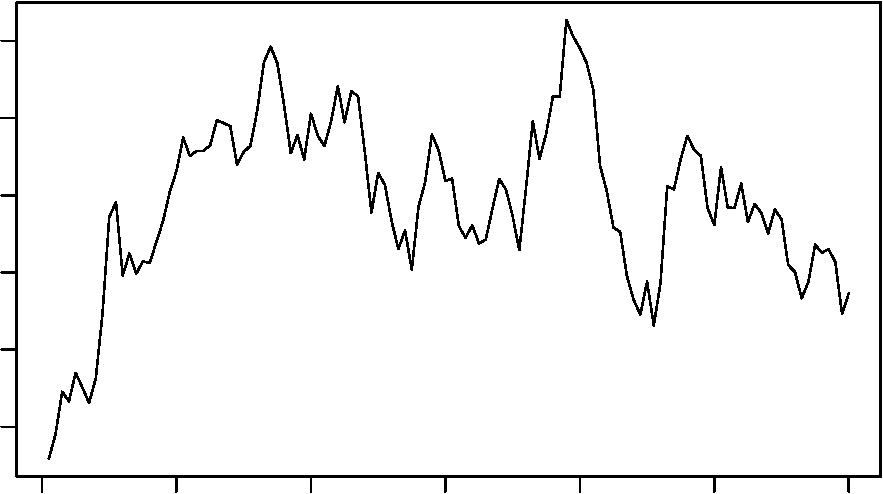
\includegraphics[width=0.8\linewidth]{Timeseries_Analysis_HW4_files/figure-latex/unnamed-chunk-5-1} \end{center}

\begin{Shaded}
\begin{Highlighting}[]
\NormalTok{acf.df10 }\OtherTok{=} \FunctionTok{acf}\NormalTok{(}\AttributeTok{x =}\NormalTok{ df10, }\AttributeTok{type =} \StringTok{"covariance"}\NormalTok{)}
\end{Highlighting}
\end{Shaded}

\begin{center}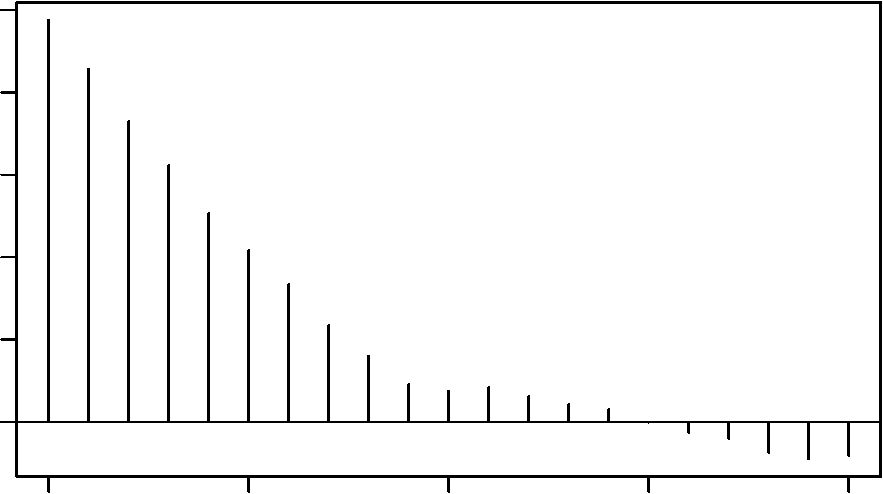
\includegraphics[width=0.8\linewidth]{Timeseries_Analysis_HW4_files/figure-latex/unnamed-chunk-5-2} \end{center}

시계열도와 SACF를 통해 비정상성을 의심하는 정도는 가능하지만,
정상시게열일 가능성을 배제할 수 없다. 추가적인 단위근검정이 필요해
보인다.

\subsection{(2)}\label{section-1}

\begin{Shaded}
\begin{Highlighting}[]
\FunctionTok{adf.test}\NormalTok{(df10, }\AttributeTok{alternative =} \StringTok{\textquotesingle{}stationary\textquotesingle{}}\NormalTok{)}
\end{Highlighting}
\end{Shaded}

\begin{verbatim}
## 
##  Augmented Dickey-Fuller Test
## 
## data:  df10
## Dickey-Fuller = -3.0271, Lag order = 4, p-value = 0.15
## alternative hypothesis: stationary
\end{verbatim}

해당 시계열이 정상시계열이라고 하기 어렵다.

\subsection{(3)}\label{section-2}

\begin{Shaded}
\begin{Highlighting}[]
\FunctionTok{adf.test}\NormalTok{(}\FunctionTok{diff}\NormalTok{(df10))}
\end{Highlighting}
\end{Shaded}

\begin{verbatim}
## Warning in adf.test(diff(df10)): p-value smaller than printed p-value
\end{verbatim}

\begin{verbatim}
## 
##  Augmented Dickey-Fuller Test
## 
## data:  diff(df10)
## Dickey-Fuller = -5.4477, Lag order = 4, p-value = 0.01
## alternative hypothesis: stationary
\end{verbatim}

1회 차분함으로써 정상시계열이 될 수 있다.

\begin{Shaded}
\begin{Highlighting}[]
\FunctionTok{auto.arima}\NormalTok{(df10, }\AttributeTok{d =} \DecValTok{1}\NormalTok{, }\AttributeTok{trace =} \ConstantTok{TRUE}\NormalTok{)}
\end{Highlighting}
\end{Shaded}

\begin{verbatim}
## 
##  ARIMA(2,1,2) with drift         : Inf
##  ARIMA(0,1,0) with drift         : 312.1437
##  ARIMA(1,1,0) with drift         : 313.4298
##  ARIMA(0,1,1) with drift         : 313.3855
##  ARIMA(0,1,0)                    : 310.2727
##  ARIMA(1,1,1) with drift         : Inf
## 
##  Best model: ARIMA(0,1,0)
\end{verbatim}

\begin{verbatim}
## Series: df10 
## ARIMA(0,1,0) 
## 
## sigma^2 = 0.7807:  log likelihood = -154.12
## AIC=310.24   AICc=310.27   BIC=313.02
\end{verbatim}

\begin{Shaded}
\begin{Highlighting}[]
\NormalTok{model }\OtherTok{\textless{}{-}} \FunctionTok{arima}\NormalTok{(df10, }\AttributeTok{order =} \FunctionTok{c}\NormalTok{(}\DecValTok{0}\NormalTok{,}\DecValTok{1}\NormalTok{,}\DecValTok{0}\NormalTok{))}
\end{Highlighting}
\end{Shaded}

ARIMA(0, 1, 0)을 채택하였다. 차분을 한 번 하는 랜덤워크이다.

\subsection{(4)}\label{section-3}

\begin{Shaded}
\begin{Highlighting}[]
\FunctionTok{checkresiduals}\NormalTok{(model)}
\end{Highlighting}
\end{Shaded}

\begin{center}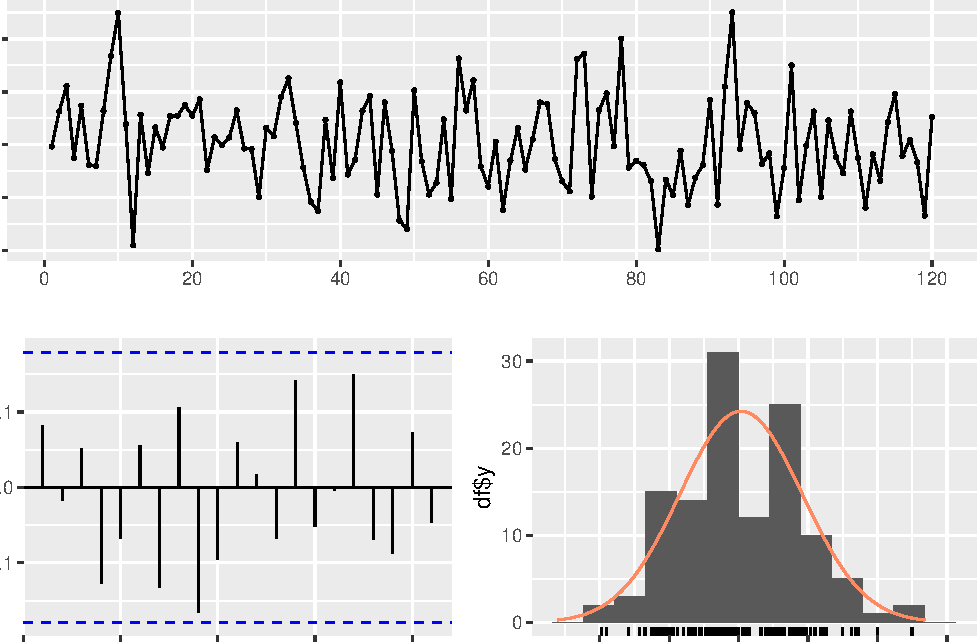
\includegraphics[width=0.8\linewidth]{Timeseries_Analysis_HW4_files/figure-latex/unnamed-chunk-9-1} \end{center}

\begin{verbatim}
## 
##  Ljung-Box test
## 
## data:  Residuals from ARIMA(0,1,0)
## Q* = 12.852, df = 10, p-value = 0.2321
## 
## Model df: 0.   Total lags used: 10
\end{verbatim}

\begin{Shaded}
\begin{Highlighting}[]
\FunctionTok{arima}\NormalTok{(df10, }\AttributeTok{order =} \FunctionTok{c}\NormalTok{(}\DecValTok{1}\NormalTok{,}\DecValTok{1}\NormalTok{,}\DecValTok{0}\NormalTok{))}
\end{Highlighting}
\end{Shaded}

\begin{verbatim}
## 
## Call:
## arima(x = df10, order = c(1, 1, 0))
## 
## Coefficients:
##          ar1
##       0.0839
## s.e.  0.0913
## 
## sigma^2 estimated as 0.7751:  log likelihood = -153.7,  aic = 311.4
\end{verbatim}

\begin{Shaded}
\begin{Highlighting}[]
\FunctionTok{arima}\NormalTok{(df10, }\AttributeTok{order =} \FunctionTok{c}\NormalTok{(}\DecValTok{0}\NormalTok{,}\DecValTok{1}\NormalTok{,}\DecValTok{1}\NormalTok{))}
\end{Highlighting}
\end{Shaded}

\begin{verbatim}
## 
## Call:
## arima(x = df10, order = c(0, 1, 1))
## 
## Coefficients:
##          ma1
##       0.0889
## s.e.  0.0947
## 
## sigma^2 estimated as 0.7748:  log likelihood = -153.68,  aic = 311.35
\end{verbatim}

잔차분석 및 과적합 진단 결과 ARIMA(1, 1, 0)과 ARIMA(0, 1, 1) 모두 계수가
낮아 유의성을 말하기 어렵다. 잔차의 형태 역시 적절하다.

\section{Q.13}\label{q.13}

\subsection{data load}\label{data-load-1}

\begin{Shaded}
\begin{Highlighting}[]
\NormalTok{gld }\OtherTok{\textless{}{-}} \FunctionTok{read\_csv}\NormalTok{(}\StringTok{\textquotesingle{}ex\_ch4\_13\_gold.csv\textquotesingle{}}\NormalTok{)}
\end{Highlighting}
\end{Shaded}

\begin{verbatim}
## Rows: 474 Columns: 2
## -- Column specification --------------------------------------------------------
## Delimiter: ","
## num  (1): price
## date (1): date
## 
## i Use `spec()` to retrieve the full column specification for this data.
## i Specify the column types or set `show_col_types = FALSE` to quiet this message.
\end{verbatim}

\begin{Shaded}
\begin{Highlighting}[]
\NormalTok{gld}\SpecialCharTok{$}\NormalTok{date }\OtherTok{\textless{}{-}} \FunctionTok{as\_date}\NormalTok{(gld}\SpecialCharTok{$}\NormalTok{date)}
\NormalTok{gld}
\end{Highlighting}
\end{Shaded}

\begin{verbatim}
## # A tibble: 474 x 2
##    date       price
##    <date>     <dbl>
##  1 2015-01-04 1216.
##  2 2015-01-11 1277.
##  3 2015-01-18 1293.
##  4 2015-01-25 1279.
##  5 2015-02-01 1235.
##  6 2015-02-08 1227.
##  7 2015-02-15 1205.
##  8 2015-02-22 1213.
##  9 2015-03-01 1164.
## 10 2015-03-08 1152.
## # i 464 more rows
\end{verbatim}

\begin{Shaded}
\begin{Highlighting}[]
\NormalTok{gold }\OtherTok{\textless{}{-}} \FunctionTok{xts}\NormalTok{(gld}\SpecialCharTok{$}\NormalTok{price, }\AttributeTok{order.by =}\NormalTok{ gld}\SpecialCharTok{$}\NormalTok{date, }\AttributeTok{col.names =} \StringTok{\textquotesingle{}price\textquotesingle{}}\NormalTok{)}
\end{Highlighting}
\end{Shaded}

\subsection{(1)}\label{section-4}

\begin{Shaded}
\begin{Highlighting}[]
\FunctionTok{plot}\NormalTok{(gold)}
\end{Highlighting}
\end{Shaded}

\begin{center}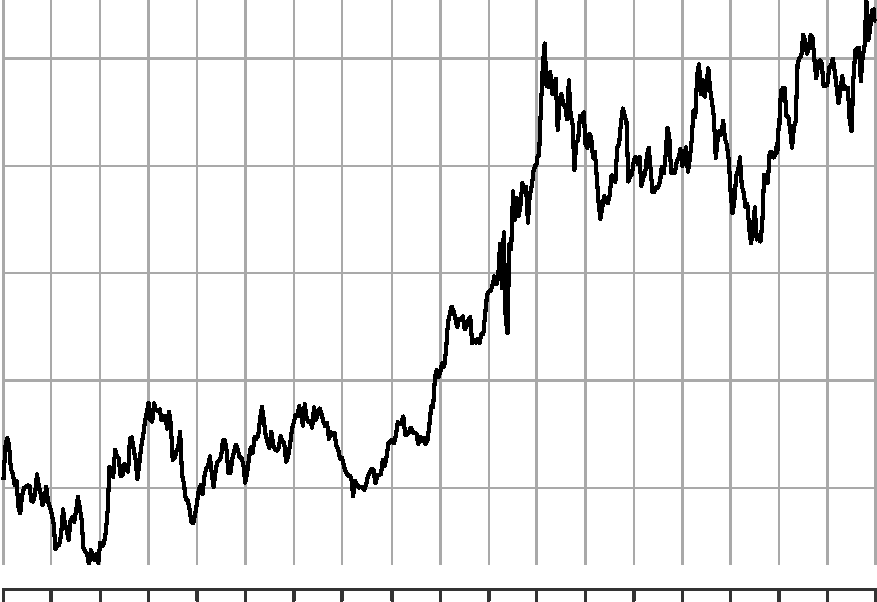
\includegraphics[width=0.8\linewidth]{Timeseries_Analysis_HW4_files/figure-latex/unnamed-chunk-11-1} \end{center}

\begin{Shaded}
\begin{Highlighting}[]
\FunctionTok{acf}\NormalTok{(gold)}
\end{Highlighting}
\end{Shaded}

\begin{center}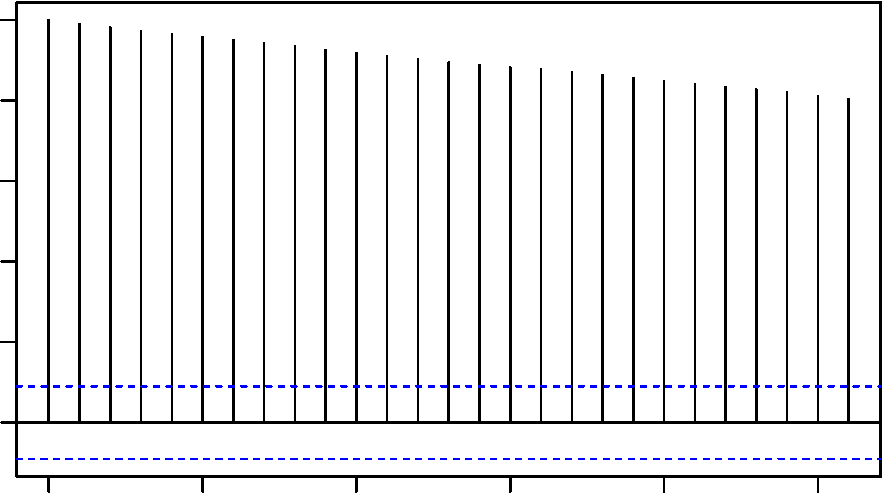
\includegraphics[width=0.8\linewidth]{Timeseries_Analysis_HW4_files/figure-latex/unnamed-chunk-11-2} \end{center}

\begin{Shaded}
\begin{Highlighting}[]
\FunctionTok{adf.test}\NormalTok{(}\AttributeTok{x =}\NormalTok{ gold, }\AttributeTok{alternative =} \StringTok{"stationary"}\NormalTok{)}
\end{Highlighting}
\end{Shaded}

\begin{verbatim}
## 
##  Augmented Dickey-Fuller Test
## 
## data:  gold
## Dickey-Fuller = -2.8001, Lag order = 7, p-value = 0.2396
## alternative hypothesis: stationary
\end{verbatim}

plot상 증가 추세가 있고, ACF가 빠르게 감소하지 않으며, ADF test를
통해서도 대립가설인 정상시계열을 기각할 수 없다. 정상시계열이라고 보기
어렵고, 차분과 로그변환을 통해 정상시계열로 만드는 것을 고려할 수 있다.

\subsection{(2)\textasciitilde(3)}\label{section-5}

차분 필요. unit root test를 통해 차분의 차수를 구한다.

여러 변환을 고려해 볼 때, 로그를 씌운 가격 데이터를 차분함으로써 분산이
일정하지는 않지만 정상시계열과 유사한 모습을 볼 수 있다. 이와 같은
데이터를 통해 auto.arima를 수행한다.

\begin{Shaded}
\begin{Highlighting}[]
\FunctionTok{plot}\NormalTok{(}\FunctionTok{BoxCox}\NormalTok{(}\AttributeTok{x =}\NormalTok{ gold, }\AttributeTok{lambda =} \FloatTok{0.2}\NormalTok{), }\AttributeTok{type =} \StringTok{"l"}\NormalTok{)}
\end{Highlighting}
\end{Shaded}

\begin{center}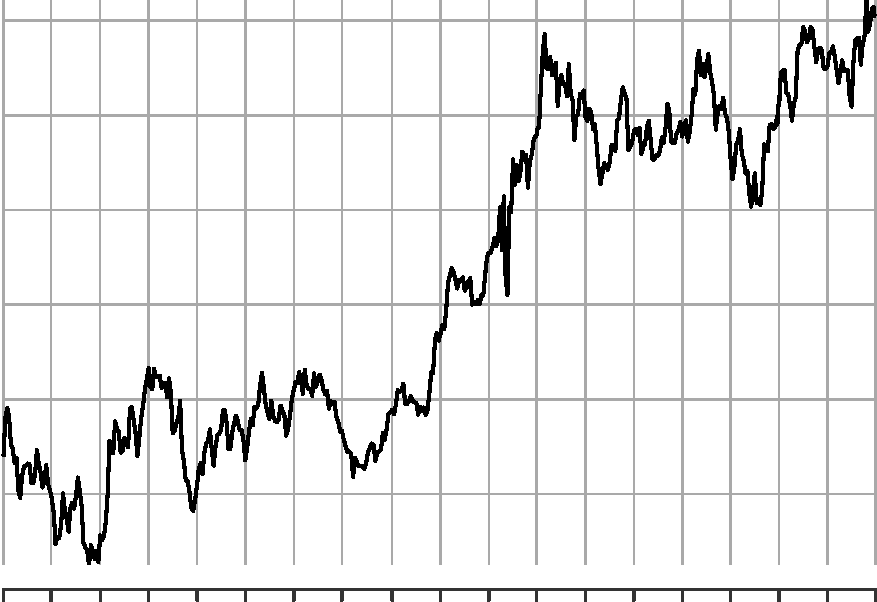
\includegraphics[width=0.8\linewidth]{Timeseries_Analysis_HW4_files/figure-latex/unnamed-chunk-12-1} \end{center}

\begin{Shaded}
\begin{Highlighting}[]
\FunctionTok{plot}\NormalTok{(}\FunctionTok{log}\NormalTok{(gold), }\AttributeTok{type =} \StringTok{"l"}\NormalTok{ )}
\end{Highlighting}
\end{Shaded}

\begin{center}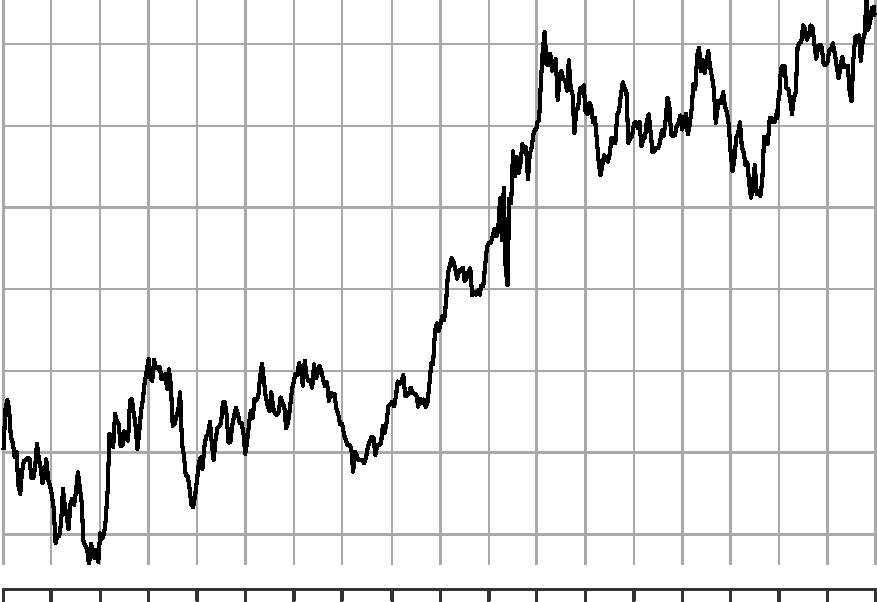
\includegraphics[width=0.8\linewidth]{Timeseries_Analysis_HW4_files/figure-latex/unnamed-chunk-12-2} \end{center}

\begin{Shaded}
\begin{Highlighting}[]
\FunctionTok{adf.test}\NormalTok{(}\AttributeTok{x =} \FunctionTok{log}\NormalTok{(gold),}
         \AttributeTok{alternative =} \StringTok{"stationary"}\NormalTok{)}
\end{Highlighting}
\end{Shaded}

\begin{verbatim}
## 
##  Augmented Dickey-Fuller Test
## 
## data:  log(gold)
## Dickey-Fuller = -2.8532, Lag order = 7, p-value = 0.2171
## alternative hypothesis: stationary
\end{verbatim}

\begin{Shaded}
\begin{Highlighting}[]
\FunctionTok{plot}\NormalTok{(}\FunctionTok{diff}\NormalTok{(}\FunctionTok{log}\NormalTok{(gold)), }\AttributeTok{type =} \StringTok{"l"}\NormalTok{)}
\end{Highlighting}
\end{Shaded}

\begin{center}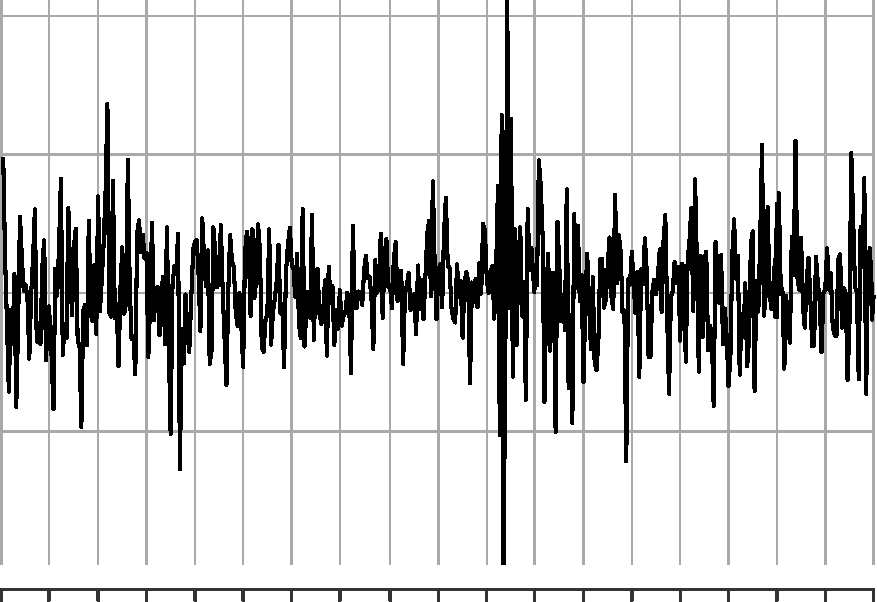
\includegraphics[width=0.8\linewidth]{Timeseries_Analysis_HW4_files/figure-latex/unnamed-chunk-12-3} \end{center}

\begin{Shaded}
\begin{Highlighting}[]
\FunctionTok{adf.test}\NormalTok{(}\AttributeTok{x =} \FunctionTok{na.omit}\NormalTok{(}\FunctionTok{diff}\NormalTok{(}\FunctionTok{log}\NormalTok{(gold))),}
         \AttributeTok{alternative =} \StringTok{"stationary"}\NormalTok{)}
\end{Highlighting}
\end{Shaded}

\begin{verbatim}
## Warning in adf.test(x = na.omit(diff(log(gold))), alternative = "stationary"):
## p-value smaller than printed p-value
\end{verbatim}

\begin{verbatim}
## 
##  Augmented Dickey-Fuller Test
## 
## data:  na.omit(diff(log(gold)))
## Dickey-Fuller = -7.8164, Lag order = 7, p-value = 0.01
## alternative hypothesis: stationary
\end{verbatim}

\begin{Shaded}
\begin{Highlighting}[]
\NormalTok{model }\OtherTok{\textless{}{-}} \FunctionTok{auto.arima}\NormalTok{(}\FunctionTok{log}\NormalTok{(gold))}
\NormalTok{model}
\end{Highlighting}
\end{Shaded}

\begin{verbatim}
## Series: log(gold) 
## ARIMA(2,1,2) with drift 
## 
## Coefficients:
##          ar1      ar2      ma1     ma2   drift
##       1.5455  -0.8529  -1.5996  0.8825  0.0011
## s.e.  0.2198   0.1350   0.2175  0.1566  0.0009
## 
## sigma^2 = 0.0004113:  log likelihood = 1175.16
## AIC=-2338.32   AICc=-2338.14   BIC=-2313.37
\end{verbatim}

\begin{Shaded}
\begin{Highlighting}[]
\FunctionTok{checkresiduals}\NormalTok{(model)}
\end{Highlighting}
\end{Shaded}

\begin{center}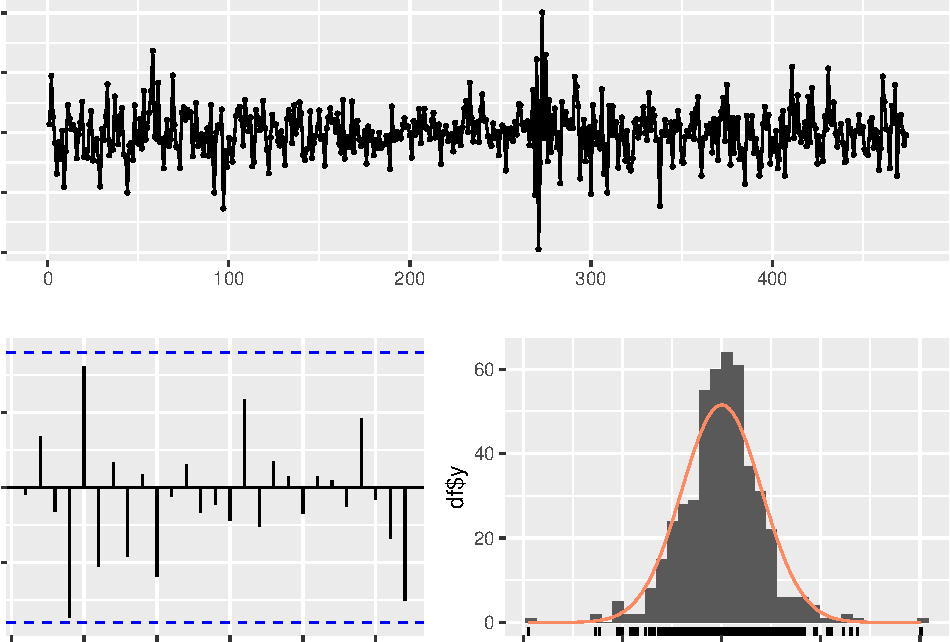
\includegraphics[width=0.8\linewidth]{Timeseries_Analysis_HW4_files/figure-latex/unnamed-chunk-13-1} \end{center}

\begin{verbatim}
## 
##  Ljung-Box test
## 
## data:  Residuals from ARIMA(2,1,2) with drift
## Q* = 11.692, df = 6, p-value = 0.06921
## 
## Model df: 4.   Total lags used: 10
\end{verbatim}

\begin{Shaded}
\begin{Highlighting}[]
\FunctionTok{arima}\NormalTok{(}\FunctionTok{log}\NormalTok{(gold), }\AttributeTok{order =} \FunctionTok{c}\NormalTok{(}\DecValTok{3}\NormalTok{,}\DecValTok{1}\NormalTok{,}\DecValTok{2}\NormalTok{))}
\end{Highlighting}
\end{Shaded}

\begin{verbatim}
## 
## Call:
## arima(x = log(gold), order = c(3, 1, 2))
## 
## Coefficients:
##          ar1      ar2      ar3      ma1     ma2
##       0.6261  -0.4344  -0.0992  -0.6791  0.4598
## s.e.  0.4168   0.2741   0.0529   0.4192  0.2799
## 
## sigma^2 estimated as 0.0004082:  log likelihood = 1174.42,  aic = -2336.84
\end{verbatim}

\begin{Shaded}
\begin{Highlighting}[]
\FunctionTok{arima}\NormalTok{(}\FunctionTok{log}\NormalTok{(gold), }\AttributeTok{order =} \FunctionTok{c}\NormalTok{(}\DecValTok{2}\NormalTok{,}\DecValTok{1}\NormalTok{,}\DecValTok{3}\NormalTok{))}
\end{Highlighting}
\end{Shaded}

\begin{verbatim}
## 
## Call:
## arima(x = log(gold), order = c(2, 1, 3))
## 
## Coefficients:
##          ar1      ar2      ma1     ma2      ma3
##       0.6310  -0.5129  -0.6846  0.5404  -0.1050
## s.e.  0.5547   0.3728   0.5526  0.3771   0.0556
## 
## sigma^2 estimated as 0.0004081:  log likelihood = 1174.49,  aic = -2336.98
\end{verbatim}

해당 자료에 대해 로그변환 후 차분 후 시계열을 만들어냄으로써 ARIMA
모델을 적합한다. ln(price) \textasciitilde{} ARIMA(2, 1, 2) 모델을
적합하였으며, 그 적절성을 잔차를 통해 검증하고 한 단계 큰 모델을 통해
확인하였다. 한 단계 큰 모델들을 검토함으로써 해당 모델의 적합성을
확인하였으나, 분산이 안정되지 않은 점 아쉽다.

\end{document}
